\documentclass[a4paper,12pt]{article}

\usepackage[margin=1in]{geometry}
\usepackage{tikz}
\usepackage{amssymb}
\usepackage{xcolor}
\usepackage{circuitikz}
\usepackage{graphicx}

\newcommand{\ra}{$\rightarrow$}
\newenvironment{6mini}{
  \begin{minipage}{6cm}
}{
  \end{minipage}
}

\title{\texttt{Logic}\\\hrulefill}
\author{Digital electronics}
\date{\small{9/6/2023}}

\begin{document}
    \maketitle

    \section{Binary Codes}
        Binary Code is how information is represented with binary digits, mulitple exist.Codes provide further implementation methods of binary into a digital system.\vspace{5pt}\\
        \textbf{Binary Coded Decimal} is code to represent decimal in binary. Each digit is represented by its binary 4-bit equivalent.\\
        \begin{6mini}
            Application include numeric LED displays. (BCD is translated digit by digit and the appropriate number is shown
            )
        \end{6mini}
        \begin{6mini}
            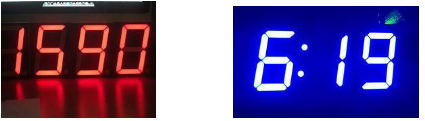
\includegraphics{LED displays.png}
        \end{6mini}
        \subsection*{Logic}
        Logic math (\texttt{Boolean Algebra}) existed before digital computers. It explained logic, by the means of math, utilizing 2 values (\textit{True or False}).
        \begin{itemize}
            \item As a transistor is a binary output, logic can be implemented
            \item Basic functions are \texttt{AND, OR, NOT}
        \end{itemize}
        \hrulefill
        \begin{itemize}
            \item \textbf{AND} \ra All inputs mus tbe true for the expression too be true. $z=xy,z=x~*~y$
            \item \textbf{OR} \ra Any 1 input can be true for the expression to be true. $z=x+y$
            \item \textbf{NOT} \ra Reverse the expression/scoped output from true to false and vice versa. $z=x'=\bar{x}$
        \end{itemize}
        \begin{center}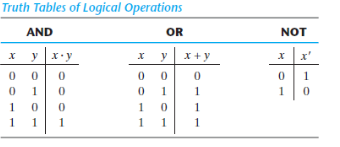
\includegraphics[width=8cm]{Truth Tables.png}\end{center}

        \subsection*{Logic gates}
            These functions are implemented with logic gates, Electronic device to implement Boolean function.
            \begin{itemize}
                \item These gatees have mulitple inputs and one output.
                \item They use specific symbols in their schematic representation
            \end{itemize}
            \begin{center}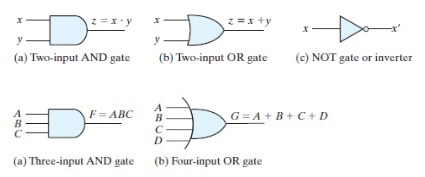
\includegraphics[width=9cm]{Logic Gates.png}\end{center}

        \subsection*{Boolean Functions}
            Varibales are used to represent inputs and outputs. in a Boolean function, ANDs appear as a product and ORs appear as a sum. NOT is represented with a ‘ or a bar above the variable.\vspace{10pt} \\
            \begin{circuitikz} \draw
                (0,4) node[not port] (not1) {}
                (4,2) node[and port] (and2) {}
                (4,4) node[and port] (and1) {}
                (not1.out) -- (and1.in 1);
            \end{circuitikz}
\end{document}